\documentclass[12pt,letterpaper]{article}

% Evidencia: GA4-220501095-AA2-EV02
% Compilar con LaTeX Workshop o: latexmk -pdf GA4-220501095-AA2-EV02.tex
% Nota: El documento usa solo caracteres ASCII para evitar problemas de codificacion.

\usepackage[spanish,es-nodecimaldot,shorthands=off]{babel}
\usepackage[T1]{fontenc}
\usepackage[utf8]{inputenc}
\usepackage{lmodern}
\usepackage{geometry}
\usepackage{setspace}
\usepackage{array}
\usepackage{longtable}
\usepackage{enumitem}
\usepackage{xcolor}
\usepackage{titlesec}
\usepackage{fancyhdr}
\usepackage{listings}
\usepackage{csquotes}
\usepackage{hyperref}
\usepackage{graphicx}
\usepackage{pdflscape}

% ==================== DATOS CONFIGURABLES ====================
\newcommand{\institucion}{Servicio Nacional de Aprendizaje -- SENA}
\newcommand{\programa}{Analisis y Desarrollo de Software}
\newcommand{\tituloTrabajo}{Informe de entregables para el proyecto de desarrollo de software}
\newcommand{\codigoEvidencia}{GA4-220501095-AA2-EV02}
\newcommand{\nombreProyecto}{Sistema de Gestion de Citas SAC}
\newcommand{\aprendiz}{Kevin Andres Granados Daza}
\newcommand{\instructor}{[Jesus Ramirez]}
\newcommand{\ficha}{[3389015]}
\newcommand{\ciudad}{Bogota D. C.}
\newcommand{\fechaEntrega}{[25 de septiembre de 2026]}
% ==============================================================

\geometry{top=2.54cm,bottom=2.54cm,left=2.54cm,right=2.54cm}
\onehalfspacing
\setlength{\parindent}{1.27cm}
\setlength{\parskip}{0pt}
\setlength{\headheight}{15pt}

\pagestyle{fancy}
\fancyhf{}
\fancyhead[L]{\codigoEvidencia}
\fancyhead[R]{\thepage}
\renewcommand{\headrulewidth}{0pt}

\titleformat{\section}{\normalfont\Large\bfseries\centering}{\thesection.}{0.5em}{}
\titleformat{\subsection}{\normalfont\large\bfseries}{\thesubsection.}{0.5em}{}

\definecolor{fondoCodigo}{RGB}{245,245,245}
\definecolor{azulCodigo}{RGB}{0,70,140}
\lstset{
    backgroundcolor=\color{fondoCodigo},
    basicstyle=\ttfamily\small,
    breaklines=true,
    frame=single,
    numbers=left,
    numberstyle=\tiny,
    keywordstyle=\color{azulCodigo}\bfseries,
    showstringspaces=false,
    tabsize=4,
    xleftmargin=0.5cm,
    xrightmargin=0.5cm
}

\begin{document}

\begin{titlepage}
    \centering
    \vspace*{2.5cm}
    {\Large \tituloTrabajo\par}
    \vspace{0.8cm}
    {\large Proyecto: \nombreProyecto\par}
    \vfill
    {\large \aprendiz\par}
    \vspace{1.5cm}
    {\large \institucion\par}
    {\large \programa\par}
    \vspace{1cm}
    {\large Evidencia: \codigoEvidencia\par}
    \vspace{1cm}
    {\large Instructor(a): \instructor\par}
    {\large Ficha: \ficha\par}
    \vfill
    {\large \ciudad\par}
    {\large \fechaEntrega\par}
\end{titlepage}

\section{Introduccion}

En un proyecto de desarrollo de software, los entregables son productos verificables que permiten evidenciar el avance del trabajo y facilitan la comunicacion entre el cliente, los usuarios y el equipo de desarrollo. Estos productos pueden corresponder a documentos, diagramas, prototipos, codigo fuente, pruebas, manuales o registros de control. Cada entregable debe tener un objetivo definido, una fuente de informacion, un responsable y un estado que permita conocer su nivel de avance.

El presente informe identifica los entregables necesarios para el proyecto \nombreProyecto. Este sistema se plantea como una aplicacion web para centralizar la gestion de citas, horarios y disponibilidad de servicios. La solucion busca disminuir tareas manuales, evitar duplicidad de informacion, mejorar la trazabilidad de las solicitudes y reducir los tiempos de espera de los usuarios.

El documento presenta el analisis de las caracteristicas principales del software, las plataformas tecnologicas propuestas para su desarrollo y los entregables de diseno que se requieren para construir el sistema aplicando los conceptos y principios de la programacion orientada a objetos. De esta forma, se establece una guia organizada para pasar de los requisitos iniciales a un producto de software funcional, verificable y mantenible.

\section{Descripcion del proyecto}

\subsection{Nombre y proposito}

El proyecto se denomina \nombreProyecto. Su proposito es desarrollar una plataforma web que permita administrar de manera centralizada la programacion de citas, la disponibilidad de horarios y el seguimiento de las solicitudes realizadas por los usuarios.

Actualmente, la gestion manual o mediante herramientas no integradas puede generar reprocesos, cruces de horario, falta de informacion actualizada y dificultades para consultar el historial de atencion. El sistema propuesto responde a esta necesidad mediante una herramienta que registra los datos de forma persistente, valida la disponibilidad y permite controlar los estados de cada cita.

\subsection{Usuarios involucrados}

El sistema contempla los siguientes tipos de usuario:

\begin{itemize}[leftmargin=1.2cm]
    \item \textbf{Usuario:} persona que se registra en la plataforma, consulta horarios y solicita, cancela o reprograma sus citas.
    \item \textbf{Administrador:} responsable de configurar horarios, consultar las citas registradas, confirmar o rechazar solicitudes y actualizar sus estados.
    \item \textbf{Sistema:} componente que valida la informacion, controla las reglas de negocio, almacena los datos y presenta mensajes segun cada proceso.
\end{itemize}

\subsection{Alcance funcional}

El alcance funcional definido para la primera version del Sistema de Gestion de Citas SAC incluye:

\begin{itemize}[leftmargin=1.2cm]
    \item Registro de usuarios e inicio de sesion.
    \item Control de acceso segun el rol asignado.
    \item Consulta de horarios disponibles.
    \item Agendamiento de citas.
    \item Cancelacion y reprogramacion de citas.
    \item Gestion de horarios por parte del administrador.
    \item Visualizacion de citas registradas y pendientes.
    \item Confirmacion, rechazo y actualizacion del estado de las citas.
    \item Almacenamiento persistente de usuarios, horarios y citas.
    \item Generacion de notificaciones o mensajes de confirmacion para las acciones realizadas.
\end{itemize}

\section{Analisis de caracteristicas del software}

\subsection{Caracteristicas funcionales}

Las caracteristicas funcionales describen las acciones que el sistema debe permitir realizar. Para este proyecto, las funciones se agrupan en los siguientes modulos:

\begin{longtable}{|p{3.3cm}|p{5.2cm}|p{6.2cm}|}
\hline
\textbf{Modulo} & \textbf{Caracteristica} & \textbf{Descripcion} \\
\hline
\endfirsthead
\hline
\textbf{Modulo} & \textbf{Caracteristica} & \textbf{Descripcion} \\
\hline
\endhead
\hline
\endfoot
\hline
\endlastfoot

Gestion de usuarios & Registro y autenticacion & Permite crear cuentas, validar datos de registro e iniciar sesion mediante correo y contrasena. \\
\hline
Control de acceso & Roles y permisos & Diferencia las opciones disponibles para usuario y administrador, evitando accesos no autorizados. \\
\hline
Agenda y disponibilidad & Consulta de horarios & Permite al usuario visualizar solamente los horarios habilitados para solicitar una cita. \\
\hline
Gestion de citas & Agendamiento & Permite seleccionar un horario disponible, validar su estado y registrar una solicitud de cita. \\
\hline
Gestion de citas & Cancelacion y reprogramacion & Permite liberar un horario cuando una cita se cancela o actualizar la fecha y hora cuando se reprograma. \\
\hline
Administracion & Gestion de horarios & Permite al administrador crear, modificar, habilitar o deshabilitar horarios de atencion. \\
\hline
Administracion & Gestion de solicitudes & Permite visualizar, confirmar, rechazar o cambiar el estado de una cita registrada. \\
\hline
Trazabilidad & Historial y estados & Conserva el registro de las acciones realizadas sobre una cita para facilitar su consulta y seguimiento. \\
\hline
Notificaciones & Mensajes de confirmacion & Informa al usuario sobre el resultado de acciones como registro, agendamiento, cancelacion o reprogramacion. \\
\hline
\end{longtable}

\subsection{Caracteristicas no funcionales}

Ademas de las funciones principales, el sistema debe cumplir condiciones de calidad que permitan una operacion confiable y adecuada:

\begin{itemize}[leftmargin=1.2cm]
    \item \textbf{Usabilidad:} la interfaz debe ser clara, intuitiva y comprensible para usuarios sin conocimientos tecnicos.
    \item \textbf{Seguridad:} el acceso debe requerir autenticacion; las contrasenas no deben almacenarse en texto plano y los permisos deben depender del rol.
    \item \textbf{Disponibilidad:} la aplicacion debe estar disponible desde navegadores modernos y dispositivos con conexion a internet.
    \item \textbf{Rendimiento:} las operaciones habituales, como consultar horarios o registrar una cita, deben responder en un tiempo adecuado para el usuario.
    \item \textbf{Persistencia:} los datos de usuarios, horarios y citas deben almacenarse de manera permanente en una base de datos.
    \item \textbf{Mantenibilidad:} el codigo debe organizarse por componentes, responsabilidades y modulos para facilitar futuros cambios.
    \item \textbf{Escalabilidad:} la solucion debe permitir agregar nuevos modulos, reportes o integraciones sin reconstruir todo el sistema.
    \item \textbf{Compatibilidad:} debe funcionar en navegadores actuales y adaptarse a pantallas de computador, tableta y telefono movil.
\end{itemize}

\section{Plataformas tecnologicas propuestas}

El Sistema de Gestion de Citas SAC se plantea como una aplicacion web con arquitectura cliente-servidor. Esta alternativa permite acceder al sistema desde un navegador sin instalar aplicaciones adicionales en los dispositivos de los usuarios.

\begin{longtable}{|p{3.2cm}|p{4cm}|p{7.5cm}|}
\hline
\textbf{Capa o recurso} & \textbf{Tecnologia propuesta} & \textbf{Justificacion de uso} \\
\hline
\endfirsthead
\hline
\textbf{Capa o recurso} & \textbf{Tecnologia propuesta} & \textbf{Justificacion de uso} \\
\hline
\endhead
\hline
\endfoot
\hline
\endlastfoot

Interfaz de usuario & HTML5, CSS3 y JavaScript & Permiten construir formularios, pantallas responsivas, calendarios, paneles y validaciones basicas en el navegador. \\
\hline
Backend & Python con framework web & Permite implementar la logica de negocio, autenticacion, validaciones, servicios y una API REST para conectar el frontend con la base de datos. \\
\hline
Base de datos & PostgreSQL o MySQL & Permiten almacenar datos estructurados de usuarios, roles, horarios, citas y estados, manteniendo integridad y relaciones entre registros. \\
\hline
API & REST con JSON & Facilita la comunicacion entre cliente y servidor mediante solicitudes estandarizadas para crear, consultar, actualizar o eliminar informacion. \\
\hline
Control de versiones & Git y GitHub & Permiten conservar el historial de cambios, respaldar el codigo y organizar las evidencias tecnicas del proyecto. \\
\hline
Entorno de desarrollo & Visual Studio Code & Facilita la edicion de codigo, el uso de terminal, la integracion con Git y la instalacion de extensiones necesarias. \\
\hline
Modelado y diagramas & Draw.io & Permite elaborar diagramas de casos de uso, clases, actividad y otros modelos UML necesarios para documentar el sistema. \\
\hline
Pruebas de servicios & Postman & Permite probar endpoints de la API, verificar respuestas y documentar solicitudes de prueba. \\
\hline
Despliegue & VPS o servicio en la nube & Permite publicar la aplicacion para que sea accesible desde internet, con posibilidad de crecimiento y copias de seguridad. \\
\hline
\end{longtable}

La seleccion de estas tecnologias se ajusta a las condiciones del proyecto porque permite una solucion web accesible, con base de datos centralizada, control de roles y posibilidad de crecimiento. Python ofrece una alternativa adecuada para aplicar programacion orientada a objetos en la capa de negocio, mientras que una base de datos relacional ayuda a conservar la consistencia de los datos de citas y horarios.

\section{Entregables del proyecto}

Los entregables son productos tangibles que evidencian el avance de cada fase del proyecto. Para cada uno se define una descripcion, estados posibles y una fuente de informacion o producto de origen.

\begin{longtable}{|p{1.2cm}|p{3.2cm}|p{5.4cm}|p{3.2cm}|p{3.2cm}|}
\hline
\textbf{Codigo} & \textbf{Entregable} & \textbf{Descripcion} & \textbf{Estados posibles} & \textbf{Fuente del producto} \\
\hline
\endfirsthead
\hline
\textbf{Codigo} & \textbf{Entregable} & \textbf{Descripcion} & \textbf{Estados posibles} & \textbf{Fuente del producto} \\
\hline
\endhead
\hline
\endfoot
\hline
\endlastfoot

E01 & Especificacion de requisitos & Documento que define requisitos funcionales, no funcionales, actores, restricciones, alcance y criterios de aceptacion del sistema. & Borrador, revisado, validado, aprobado, actualizado. & Cliente, usuarios, entrevistas y analisis del proyecto. \\
\hline

E02 & Historias de usuario & Descripcion de necesidades desde la perspectiva de usuario, administrador o sistema, con prioridad y criterios de aceptacion. & Pendiente, elaborada, priorizada, validada, implementada. & Requisitos funcionales y necesidades de los usuarios. \\
\hline

E03 & Catalogo de casos de uso & Plantillas que detallan los flujos normal y alternativo de registro, inicio de sesion, agendamiento y gestion de citas. & Borrador, revisado, aprobado, actualizado. & Requisitos funcionales e historias de usuario. \\
\hline

E04 & Diagrama de casos de uso & Modelo UML que representa los actores externos y las funcionalidades principales del sistema. & En diseno, revisado, validado, aprobado. & Catalogo de casos de uso. \\
\hline

E05 & Diagrama de clases & Modelo estructural que define clases, atributos, metodos, relaciones y responsabilidades del sistema. & Borrador, revisado, aprobado, implementado. & Modelo de dominio, requisitos y principios POO. \\
\hline

E06 & Diagramas de actividad & Representacion de los flujos de inicio de sesion, registro, agendamiento, cancelacion, reprogramacion y gestion administrativa. & Pendiente, elaborado, revisado, aprobado. & Casos de uso y reglas de negocio. \\
\hline

E07 & Diseno de base de datos & Modelo de entidades, relaciones, llaves y reglas de integridad para usuarios, horarios, citas, roles y estados. & Borrador, validado, implementado, actualizado. & Diagrama de clases, requisitos y reglas de negocio. \\
\hline

E08 & Registro de trazabilidad & Matriz que relaciona cada requisito con historias de usuario, casos de uso, clases, pruebas y resultados. & Inicial, actualizado, verificado, cerrado. & Todos los artefactos del proyecto. \\
\hline

E09 & Prototipo de interfaz & Bocetos o pantallas de registro, inicio de sesion, agenda, formulario de cita y panel administrativo. & Boceto, en revision, validado, aprobado. & Requisitos de usuario y diseno de interfaz. \\
\hline

E10 & Codigo fuente & Implementacion del frontend, backend, modelos, controladores, servicios y configuracion de la aplicacion. & En desarrollo, en prueba, corregido, versionado, liberado. & Diagramas de diseno y requisitos aprobados. \\
\hline

E11 & Casos de prueba & Escenarios con precondiciones, datos de entrada, pasos, resultado esperado y resultado obtenido. & Disenado, ejecutado, aprobado, fallido, corregido. & Requisitos, historias de usuario y casos de uso. \\
\hline

E12 & Reporte de pruebas & Documento que consolida las pruebas ejecutadas, incidencias encontradas, correcciones y estado de calidad. & Preliminar, revisado, aprobado, cerrado. & Casos de prueba y ejecucion del sistema. \\
\hline

E13 & Manual de usuario & Guia para que el usuario se registre, inicie sesion, consulte horarios y gestione sus citas. & Borrador, revisado, publicado, actualizado. & Sistema funcional y retroalimentacion de usuarios. \\
\hline

E14 & Manual tecnico & Documento para instalacion, configuracion, arquitectura, base de datos, despliegue y mantenimiento de la aplicacion. & Borrador, revisado, entregado, actualizado. & Codigo fuente, configuracion e infraestructura. \\
\hline
\end{longtable}

\section{Entregables de diseno orientado a objetos}

La programacion orientada a objetos permite organizar el sistema mediante clases que representan entidades reales del dominio de las citas. Cada clase agrupa datos y comportamientos relacionados, lo cual facilita la reutilizacion, el mantenimiento y la escalabilidad del software.

\subsection{Clases principales identificadas}

\begin{longtable}{|p{3cm}|p{4.5cm}|p{4.5cm}|p{4.2cm}|}
\hline
\textbf{Clase} & \textbf{Responsabilidad} & \textbf{Atributos principales} & \textbf{Metodos principales} \\
\hline
\endfirsthead
\hline
\textbf{Clase} & \textbf{Responsabilidad} & \textbf{Atributos principales} & \textbf{Metodos principales} \\
\hline
\endhead
\hline
\endfoot
\hline
\endlastfoot

Usuario & Representa a la persona que utiliza el sistema para solicitar y gestionar citas. & id, nombre, correo, contrasena, estado. & registrarse(), iniciarSesion(), agendarCita(), cancelarCita(), reprogramarCita(). \\
\hline

Administrador & Representa al usuario con permisos para administrar horarios y solicitudes de cita. & id, nombre, correo, rol. & gestionarHorarios(), visualizarCitas(), confirmarCita(), rechazarCita(). \\
\hline

Horario & Representa una franja de tiempo disponible o no disponible para prestar un servicio. & id, fecha, horaInicio, horaFin, disponible. & verificarDisponibilidad(), habilitar(), deshabilitar(). \\
\hline

Cita & Representa una solicitud de atencion asociada a un usuario y un horario. & id, fecha, hora, estado, usuario, horario. & crear(), confirmar(), cancelar(), reprogramar(), cambiarEstado(). \\
\hline

Notificacion & Representa un mensaje generado por el sistema para informar una accion o cambio de estado. & id, mensaje, fechaEnvio, leida. & enviar(), marcarComoLeida(). \\
\hline
\end{longtable}

\subsection{Aplicacion de los principios POO}

\begin{itemize}[leftmargin=1.2cm]
    \item \textbf{Abstraccion:} cada clase representa solamente la informacion y acciones necesarias para el sistema. Por ejemplo, la clase Cita concentra los datos relevantes de una solicitud sin incluir detalles que no aportan a la gestion de citas.
    \item \textbf{Encapsulamiento:} los atributos sensibles, como la contrasena de un usuario o el estado de una cita, deben protegerse y modificarse mediante metodos que validen las reglas de negocio.
    \item \textbf{Herencia:} la clase Administrador puede heredar los atributos comunes de Usuario, como nombre, correo y credenciales, y agregar operaciones administrativas.
    \item \textbf{Polimorfismo:} un metodo como mostrarPanel() puede comportarse de forma diferente segun el objeto. Un Usuario visualiza sus citas y horarios; un Administrador visualiza opciones de configuracion y control.
\end{itemize}

\subsection{Descripcion del diagrama de clases}

A continuacion, se presenta el diagrama entidad-relacion propuesto para el Sistema de Gestion de Citas SAC. El modelo representa las entidades principales del sistema, sus atributos, las llaves primarias y foraneas, y las relaciones necesarias para almacenar usuarios, roles, horarios, citas, notificaciones e historial de cambios.

\begin{figure}[htbp]
    \centering
    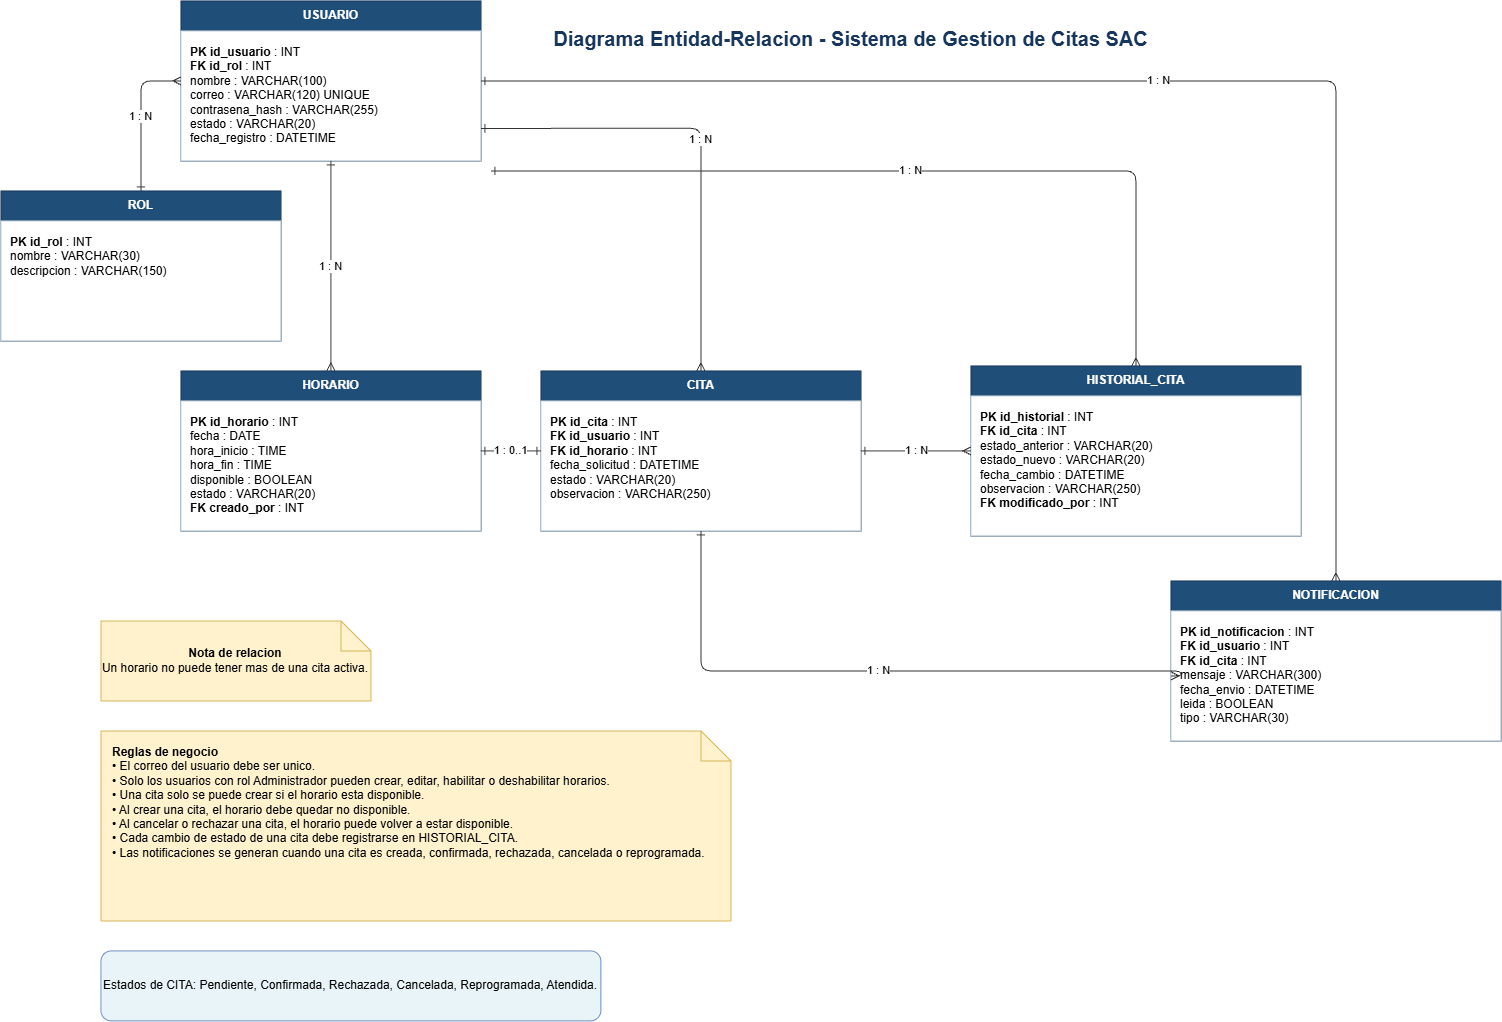
\includegraphics[width=0.90\textwidth]{Entidad Relacion.png}
    \caption{Diagrama entidad-relacion del Sistema de Gestion de Citas SAC.}
    \label{fig:diagrama-er-sac}
\end{figure}

Como se observa en la Figura~\ref{fig:diagrama-er-sac}, la entidad Usuario se relaciona con Rol, Horario, Cita, HistorialCita y Notificacion. La entidad Cita constituye el elemento central del modelo porque relaciona al usuario con un horario y permite registrar los estados, cambios y notificaciones asociados a cada solicitud.

\section{Trazabilidad de requisitos y entregables}

La trazabilidad permite comprobar que cada necesidad planteada por el cliente se refleja en un artefacto de analisis, diseno, implementacion y prueba. La siguiente matriz presenta algunos ejemplos de relacion entre requisitos y entregables.

\begin{longtable}{|p{2cm}|p{4.2cm}|p{3.4cm}|p{3.3cm}|p{3.5cm}|}
\hline
\textbf{Requisito} & \textbf{Descripcion} & \textbf{Diseno asociado} & \textbf{Prueba asociada} & \textbf{Entregable relacionado} \\
\hline
\endfirsthead
\hline
\textbf{Requisito} & \textbf{Descripcion} & \textbf{Diseno asociado} & \textbf{Prueba asociada} & \textbf{Entregable relacionado} \\
\hline
\endhead
\hline
\endfoot
\hline
\endlastfoot

RF01 & Registrar usuarios y roles. & Clase Usuario, formulario de registro y caso de uso Registrar Usuario. & Validar registro con datos correctos, incompletos y correo repetido. & E01, E02, E03, E05, E09, E11. \\
\hline

RF02 & Consultar horarios disponibles. & Clase Horario, caso de uso Consultar Horarios y pantalla de agenda. & Verificar que se muestren solo horarios habilitados. & E01, E03, E04, E05, E09, E11. \\
\hline

RF03 & Agendar una cita. & Clase Cita, relacion Usuario-Cita-Horario y caso de uso Agendar Cita. & Validar disponibilidad y registro de cita pendiente. & E01, E02, E03, E05, E07, E11. \\
\hline

RF04 & Cancelar o reprogramar una cita. & Metodos cancelar() y reprogramar() de Cita; diagramas de actividad. & Verificar actualizacion de estado y liberacion del horario. & E03, E05, E07, E11, E12. \\
\hline

RF05 & Gestionar horarios. & Clase Horario y operaciones administrativas. & Verificar creacion, edicion, habilitacion y deshabilitacion de horarios. & E01, E03, E05, E10, E11. \\
\hline

RF06 & Confirmar o rechazar citas. & Clase Administrador y metodo cambiarEstado() de Cita. & Verificar transicion entre estados pendiente, confirmada y rechazada. & E03, E05, E06, E11, E12. \\
\hline
\end{longtable}

\section{Estados generales de los entregables}

Para llevar control sobre los productos del proyecto se propone utilizar los siguientes estados generales:

\begin{itemize}[leftmargin=1.2cm]
    \item \textbf{Pendiente:} el entregable ha sido identificado, pero todavia no se inicia su elaboracion.
    \item \textbf{En elaboracion:} el equipo esta creando el contenido o artefacto correspondiente.
    \item \textbf{En revision:} el producto esta siendo evaluado por el equipo, instructor, cliente o usuario responsable.
    \item \textbf{Validado:} se comprobo que el entregable cumple con los requisitos o criterios definidos.
    \item \textbf{Aprobado:} el responsable acepta formalmente el producto para continuar con la siguiente etapa.
    \item \textbf{Actualizado:} el entregable fue modificado debido a cambios en requisitos, diseno o pruebas.
    \item \textbf{Cerrado:} el producto fue entregado y no requiere modificaciones pendientes en la version actual.
\end{itemize}

El uso de estos estados permite conocer el avance del proyecto y facilita la toma de decisiones. Por ejemplo, un caso de uso no deberia pasar a implementacion sin haber sido revisado y validado; de la misma manera, un reporte de pruebas no se debe cerrar mientras existan incidencias criticas sin corregir.

\section{Conclusiones}

El analisis realizado permite establecer que el Sistema de Gestion de Citas SAC requiere una organizacion clara de sus entregables para asegurar que las necesidades de los usuarios se transformen en una solucion de software verificable. La especificacion de requisitos, los casos de uso, los diagramas UML, el diseno de base de datos, el codigo fuente, las pruebas y los manuales son productos complementarios que permiten controlar el desarrollo desde el inicio hasta la entrega final.

Las caracteristicas identificadas muestran que el sistema debe centralizar la gestion de usuarios, horarios y citas, manteniendo control sobre los estados y permitiendo acciones como agendar, cancelar, reprogramar, confirmar o rechazar solicitudes. Estas funciones responden a la necesidad de reducir procesos manuales, mejorar la trazabilidad y ofrecer una experiencia mas organizada para usuarios y administradores.

La seleccion de una arquitectura web con frontend, backend, base de datos relacional, API REST y control de versiones permite construir una solucion accesible, mantenible y escalable. Ademas, la aplicacion de los principios de programacion orientada a objetos aporta una estructura adecuada para representar las entidades principales del proyecto y separar las responsabilidades de cada componente.

Finalmente, el registro de trazabilidad y la definicion de estados para los entregables facilitan el seguimiento del proyecto. Esto permite relacionar cada requisito con su diseno, implementacion y prueba, disminuyendo el riesgo de que una necesidad importante sea omitida durante el desarrollo del Sistema de Gestion de Citas SAC.

\end{document}
